\chapter{Product Description}

\section{Motivation}
Understanding of Intel 8085 microprocessor is fundamental to getting insight into the Von-Neumann Architecture. It was first introduced in 1976, since then many generations of computer architecture have come up, some still persists while others are lost in history. This microprocessor still survives because it is still popular in university and training institutes to get students acquainted with basic computer architecture. For this purpose 8085 trainer kit are available on the market. However, with more popular technologies to learn, technical syllabus has very low time bandwidth available for this topic. All that is necessary for the students is to understand the functional working model of this basic architecture and then proceed on to next advance level of the subject.

With this academic learning purpose in mind this simulator software is designed. It helps in get started easily with example codes, and to learn the architecture playfully. It also provides a trainer kit as an appealing functional alternative to real hardware. The users can write assembly code easily and get results quickly without even having the actual hardware. 

\section{Installation and Upgrade Note}

The program code is written Java Syntax and available in java virtual machine executable format (.jar). To run in :\\
\textbf{Windows : }\\
1)  Make sure you have Java installed on your system. Check this by typing \textbf{java -version} into the command terminal. If you don't have the latest version of Java, update it before proceeding. \\
2) Install Java (ver >6) \url{http://www.java.com/en/download/manual.jsp}\\
3) Just \textbf{double clic}k the ``.jar '' file, it should execute. \\
4) Otherwise you can execute in CMD ( Command Prompt ) by typing `` \textbf{java -jar <filename>.jar} ''\\
\\
\textbf{Linux : }\\
1) Open terminal and type `` \textbf{java -jar <filename>.jar} ''
\\
\\
\textbf{\large UPDATES : }\\
Automatic or push updates are not supported in this software. Users are requested to keep track of the new release available at the web-link :  \url{https://8085simulator.codeplex.com/}.
\section{Limitations}

This or any 8085 simulator software is no way a replacement for real hardware. It only does functional simulation of the codes. It is not an emulator and hence do not expect that the timing information will be accurately modeled. However, the exact performance of the code can only be monitored in real 8085 microprocessor hardware. 

\section{Known Issues}
\begin{itemize}
	\item Issue 1 : DAA instruction wrongly toggles the carry flag if already there is a carry instead of setting it high, like take for example (88H + 88H). Users need to be cautious while using this instruction. It will be fixed in future realize v2.1.
	 \item Issue 2: In Assembler Window, during pre-processing stage of the code it flags error if\\ ` ; ' (SEMICOLON) comment marking character is followed after `` // '' (DOUBLE FORWARD SLASH).\\
	 Example $ \rightarrow $  "<Label>: <Assembler Code> // <Comments> ; <More Comments>"
\end{itemize}

\section{Software Design Architecture}

\begin{figure}[htbp]
	\centering 
	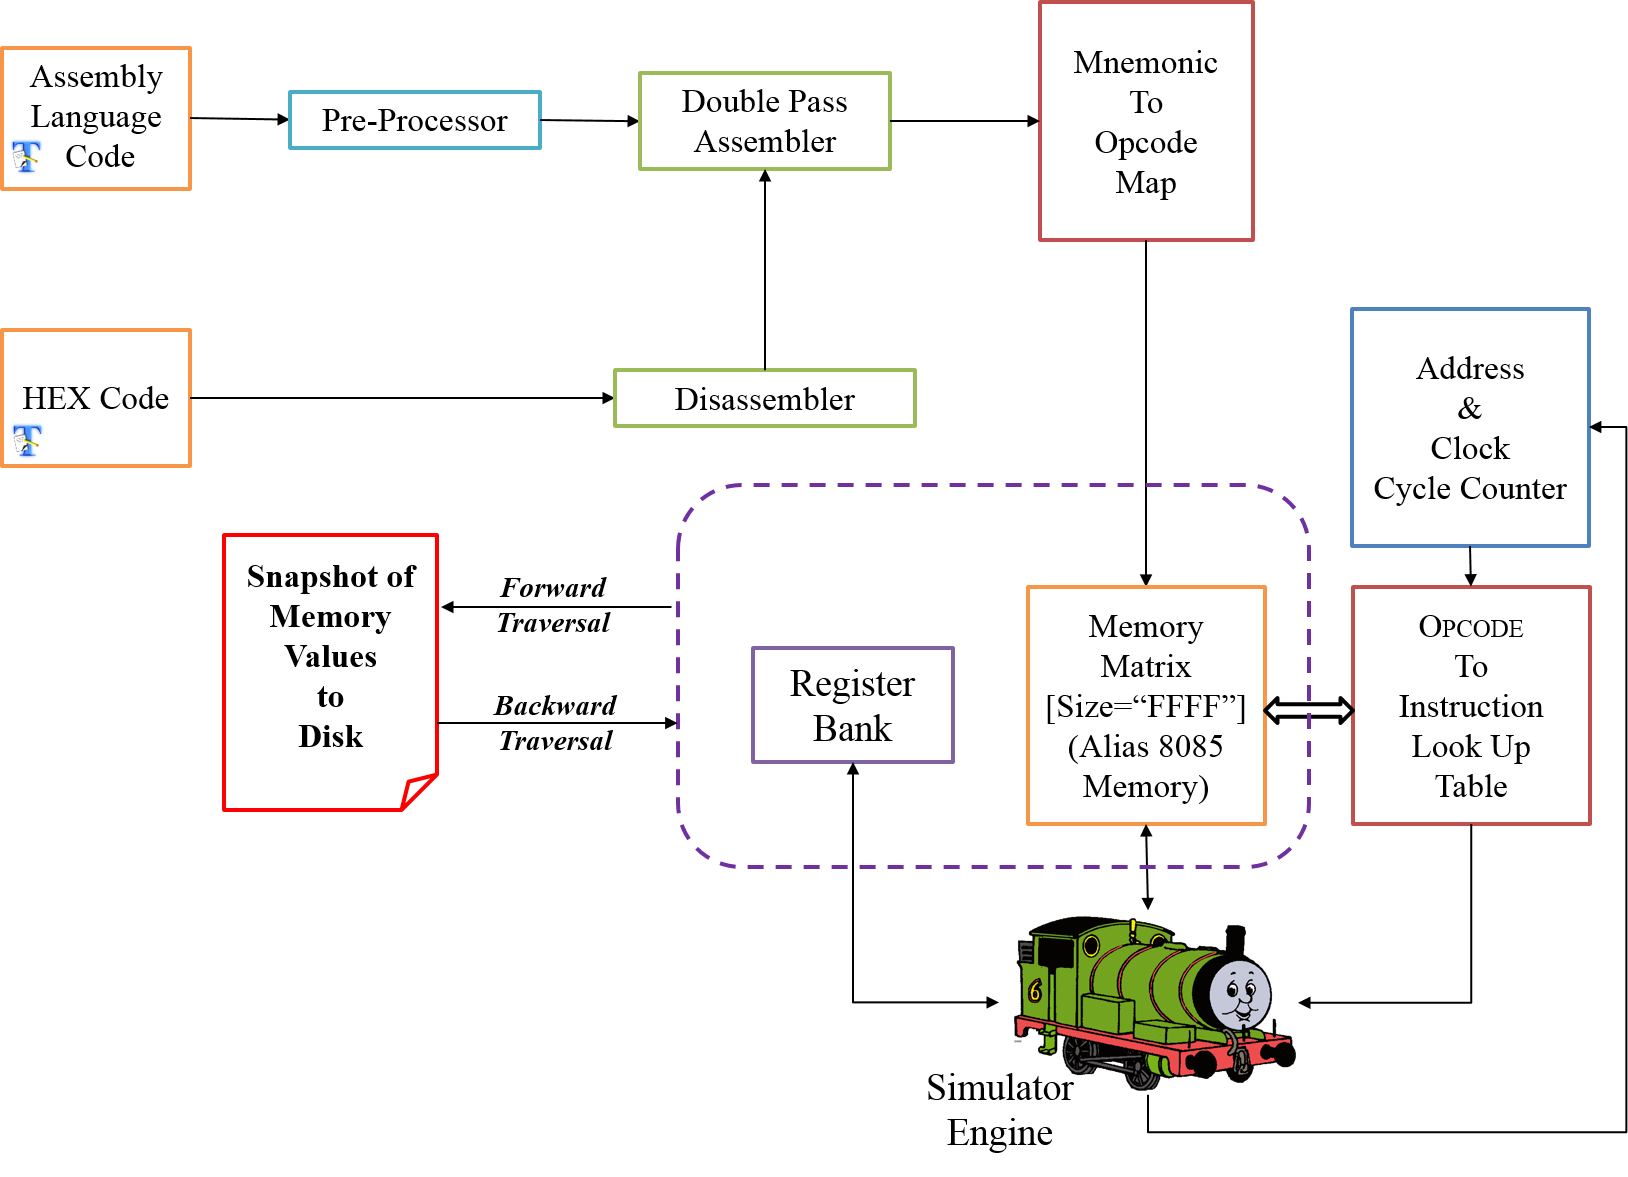
\includegraphics[width=0.9\linewidth]{./soft_arch.png}
	\caption{Software Architecture}
	\label{fig:software:architecture}
\end{figure}

\subsection{Preprocessor}
Assembler directives are lines included in the code of programs preceded by a hash sign (\#). These lines are not program statements but directives for the preprocessor. The preprocessor examines the code before actual assembling of code begins and resolves all these directives before any code is actually generated by regular statements. 

\subsection{Assembler}
It uses a 2 pass Assembler. In first pass it constructs \textit{the symbol table} in which every label of the assembly program is stored with its corresponding location. In the second pass the assembler locates (using the flags array) and completes (using the symbol table) the partial mnemonics instructions. It then convert Mnemonic to Opcode using a mapping method.

\subsection{Simulator Engine}
It resets all the register. Then starts from "Origin address". It scans the opcode value and sends it to "Opcode to instruction set look table". It then instructs the simulator engine the registers that will be affected, the number of data opcode that follows after the instruction opcode to increment the address and also to increment the number of clock cycles accordingly.

\subsection{Step-wise Traversal Controller}
It consists of \textit{memory snapshot maker} and \textit{memory register - data value monitor}. During forward traversal \textit{memory snapshot maker} dumps the entire memory current values to a temp file. With each forward step one temp file is created in the working directory pool of the software. During backward traversal the \textit{memory snapshot maker} read backs the temp files and reloads with the past value. Once the process is stopped it clears out all the snapshots that are dumped. In this manner this software can able to traverse also in backward direction, inspite of using forward traversal instruction code.

\section{Source Code}
The entire design is built in \textbf{Netbeans IDE} with JDK bundle. It can easily be opened by the software. The coding was done in bit unprofessional way, as it was developed during very early stage of my academics. Students are free to use the code for their understanding and distribution as defined under the GNU license agreement. 

%The source code for version 2 is available in the web-link : \\
%\url{https://8085simulator.codeplex.com/downloads/get/1551429}

It is being actively maintained in GIT repository find it at link :\\
\url{https://8085simulator.codeplex.com/SourceControl/latest}\\
\url{https://github.com/8085simulator/8085simulator}
%\url{https://github.com/jm61288/8085Simulator}